\documentclass[12pt]{report}
\usepackage[utf8]{inputenc}
\usepackage[russian]{babel}
%\usepackage[14pt]{extsizes}
\usepackage{listings}
\usepackage{graphicx}
\usepackage{amsmath,amsfonts,amssymb,amsthm,mathtools} 
\usepackage{pgfplots}
\usepackage{filecontents}
\usepackage{float}
\usepackage{comment}
\usepackage{indentfirst}
\usepackage{eucal}
\usepackage{pdfpages}
\usepackage{enumitem}
%s\documentclass[openany]{book}
\frenchspacing

\usepackage{indentfirst} % Красная строка

\usetikzlibrary{datavisualization}
\usetikzlibrary{datavisualization.formats.functions}

\usepackage{amsmath}


% Для листинга кода:
\lstset{ %
	language=c,                 % выбор языка для подсветки (здесь это С)
	basicstyle=\small\sffamily, % размер и начертание шрифта для подсветки кода
	numbers=left,               % где поставить нумерацию строк (слева\справа)
	numberstyle=\tiny,           % размер шрифта для номеров строк
	stepnumber=1,                   % размер шага между двумя номерами строк
	numbersep=5pt,                % как далеко отстоят номера строк от подсвечиваемого кода
	showspaces=false,            % показывать или нет пробелы специальными отступами
	showstringspaces=false,      % показывать или нет пробелы в строках
	showtabs=false,             % показывать или нет табуляцию в строках
	frame=single,              % рисовать рамку вокруг кода
	tabsize=2,                 % размер табуляции по умолчанию равен 2 пробелам
	captionpos=t,              % позиция заголовка вверху [t] или внизу [b] 
	breaklines=true,           % автоматически переносить строки (да\нет)
	breakatwhitespace=false, % переносить строки только если есть пробел
	escapeinside={\#*}{*)}   % если нужно добавить комментарии в коде
}


\usepackage[left=2cm,right=2cm, top=2cm,bottom=2cm,bindingoffset=0cm]{geometry}
% Для измененных титулов глав:
\usepackage{titlesec, blindtext, color} % подключаем нужные пакеты
\definecolor{gray75}{gray}{0.75} % определяем цвет
\newcommand{\hsp}{\hspace{20pt}} % длина линии в 20pt
% titleformat определяет стиль
\titleformat{\chapter}[hang]{\Huge\bfseries}{\thechapter\hsp\textcolor{gray75}{|}\hsp}{0pt}{\Huge\bfseries}


% plot
\usepackage{pgfplots}
\usepackage{filecontents}
\usetikzlibrary{datavisualization}
\usetikzlibrary{datavisualization.formats.functions}

\begin{document}
	%\def\chaptername{} % убирает "Глава"
	\thispagestyle{empty}
	\begin{titlepage}
		\noindent \begin{minipage}{0.15\textwidth}
			
\includegraphics[width=\linewidth]{b_logo}
		\end{minipage}
		\noindent\begin{minipage}{0.9\textwidth}\centering
			\textbf{Министерство науки и высшего образования Российской Федерации}\\
			\textbf{Федеральное государственное бюджетное образовательное учреждение высшего образования}\\
			\textbf{~~~«Московский государственный технический университет имени Н.Э.~Баумана}\\
			\textbf{(национальный исследовательский университет)»}\\
			\textbf{(МГТУ им. Н.Э.~Баумана)}
		\end{minipage}
		
		\noindent\rule{18cm}{3pt}
		\newline\newline
		\noindent ФАКУЛЬТЕТ $\underline{\text{«Информатика и системы управления»}}$ \newline\newline
		\noindent КАФЕДРА $\underline{\text{«Программное обеспечение ЭВМ и информационные технологии»}}$\newline\newline\newline\newline\newline
		
		\begin{center}
			\noindent\begin{minipage}{1.1\textwidth}\centering
				\Large\textbf{Отчет по лабораторной работе №11}\newline
				\textbf{по дисциплине <<Функциональное и логическое}\newline
				\textbf{~~~программирование>>}\newline\newline
			\end{minipage}
		\end{center}
		
		\noindent\textbf{Тема} $\underline{\text{Рекурсия на Prolog~~~~~~~~~~~~~~~~~~~~~~~~~~~~~~~~~~~~~~~~~~~~~~~~~~~~~~~~~~~~~~}}$\newline\newline
		\noindent\textbf{Студент} $\underline{\text{Золотухин А.В.~~~~~~~~~~~~~~~~~~~~~~~~~~~~~~~~~~~~~~~~~~~~~~~~~~~~~~~~~~~~~~}}$\newline\newline
		\noindent\textbf{Группа} $\underline{\text{ИУ7-64Б~~~~~~~~~~~~~~~~~~~~~~~~~~~~~~~~~~~~~~~~~~~~~~~~~~~~~~~~~~~~~~~~~~~~~~~~~}}$\newline\newline
		\noindent\textbf{Оценка (баллы)} $\underline{\text{~~~~~~~~~~~~~~~~~~~~~~~~~~~~~~~~~~~~~~~~~~~~~~~~~~~~~~~~~~~~~~~~~~~~~~~~}}$\newline\newline
		\noindent\textbf{Преподаватель} $\underline{\text{Толпинская Н.Б., Строганов Ю. В.~~~~~~~~~~~~~~~~~~~~~~~~~~}}$\newline\newline\newline
		
		\begin{center}
			\vfill
			Москва~---~\the\year
			~г.
		\end{center}
	\end{titlepage}
	
	
	\section*{Задание}
	
	Используя хвостовую рекурсию, разработать (комментируя назначение аргументов) эффективную программу, позволяющую:
	\begin{enumerate}
		\item Найти длину списка (по верхнему уровню);
		\item Найти сумму элементов числового списка;
		\item Найти сумму элементов числового списка, стоящих на нечетных позициях исходного списка (нумерация от 0);
		\item Сформировать список из элементов числового списка, больших заданного значения;
		\item Удалить заданный элемент из списка (один или все вхождения);
		\item Объединить два списка.
	\end{enumerate}
	
	\section*{Решение}
	\subsection*{1. Найти длину списка (по верхнему уровню)}
	\begin{lstlisting}	
domains
	list = integer*
	n = integer
	
predicates
	len(list, n).
	lenHelp(list, n, n).
	
clauses
	len(L, Res) :- lenHelp(L, Res, 0).
	lenHelp([], Res, Res) :- !.
	lenHelp([_|T], Res, CurLen) :- NewCurLen = CurLen + 1, 
															   lenHelp(T, Res, NewCurLen).

goal
	len([1, 2, 3], Res).
	\end{lstlisting}
	\clearpage
	\subsection*{2. Найти сумму элементов числового списка}
	\begin{lstlisting}	
domains
	list = integer*
	n = integer
	
predicates
	sum(list, n).
	sumHelp(list, n, n).
	
clauses
	sum(L, Res) :- sumHelp(L, Res, 0).
	sumHelp([], Res, Res) :- !.
	sumHelp([H|T], Res, CurSum) :- NewCurSum = CurSum + H, 
																 sumHelp (T, Res, NewCurSum).
	
goal
	sum([1, 2, 3], Res).
	\end{lstlisting}

\subsection*{3. Найти сумму элементов числового списка, стоящих на нечетных позициях исходного списка}
\begin{lstlisting}	
	domains
	list = integer*
	n = integer
	
	predicates
	sumOddPos(list, n).
	sumHelp(list, n, n).
	
	clauses
	sumOddPos(L, Res) :- sumHelp(L, Res, 0).
	sumHelp([], Res, Res) :- !.
	sumHelp([_|[]], Res, Res) :- !.
	sumHelp([_|[H|T]], Res, CurSum) :- NewCurSum = CurSum + H, 
	sumHelp(T, Res, NewCurSum).
	
	goal
	sumOddPos([1, 2, 3], Res).
\end{lstlisting}
\clearpage
\subsection*{4. Сформировать список из элементов числового списка, больших заданного значения}
\begin{lstlisting}	
	domains
	list = integer*
	n = integer
	
	predicates
	greaterThan(list, n, list).
	
	clauses
	
	greaterThan([H|T], N, [H|ResT]) :- H > N, !, greaterThan(T, N, ResT).
	greaterThan([_|T], N, Res) :- greaterThan(T, N, Res), !.
	greaterThan([], _, []).
	
	goal
	greaterThan([3, 1, 2, 3], 2, Res). 
\end{lstlisting}

\subsection*{5. Удалить заданный элемент из списка (один или все вхождения)}
\begin{lstlisting}	
domains
	list = integer*
	n = integer
	
predicates
	removeAll(list, n, list).
	removeOne(list, n, list).

clauses
	removeAll([N|T], N, ResT) :- removeAll(T, N, ResT), !.
	removeAll([H|T], N, [H|Res]) :- removeAll(T, N, Res).
	removeAll([], _,[]).

	removeOne([N|T], N, T) :- !.
	removeOne([H|T], N, [H|ResT]) :- removeOne(T, N, ResT), !.
	removeOne([], _,[]).

goal
	removeAll([1, 2, 3, 2], 2, Res).
	%removeOne([1, 2, 3, 2], 2, Res).
\end{lstlisting}
\clearpage
\subsection*{6. Объединить два списка}
\begin{lstlisting}	
domains
	list = integer*

predicates
	append(list, list, list) .
	
clauses
	append([], L, L) :- !.
	append([H|T], L, [H|ResT]) :- append(T, L, ResT).

goal
	append([1, 2], [3, 4], Res).
\end{lstlisting}
	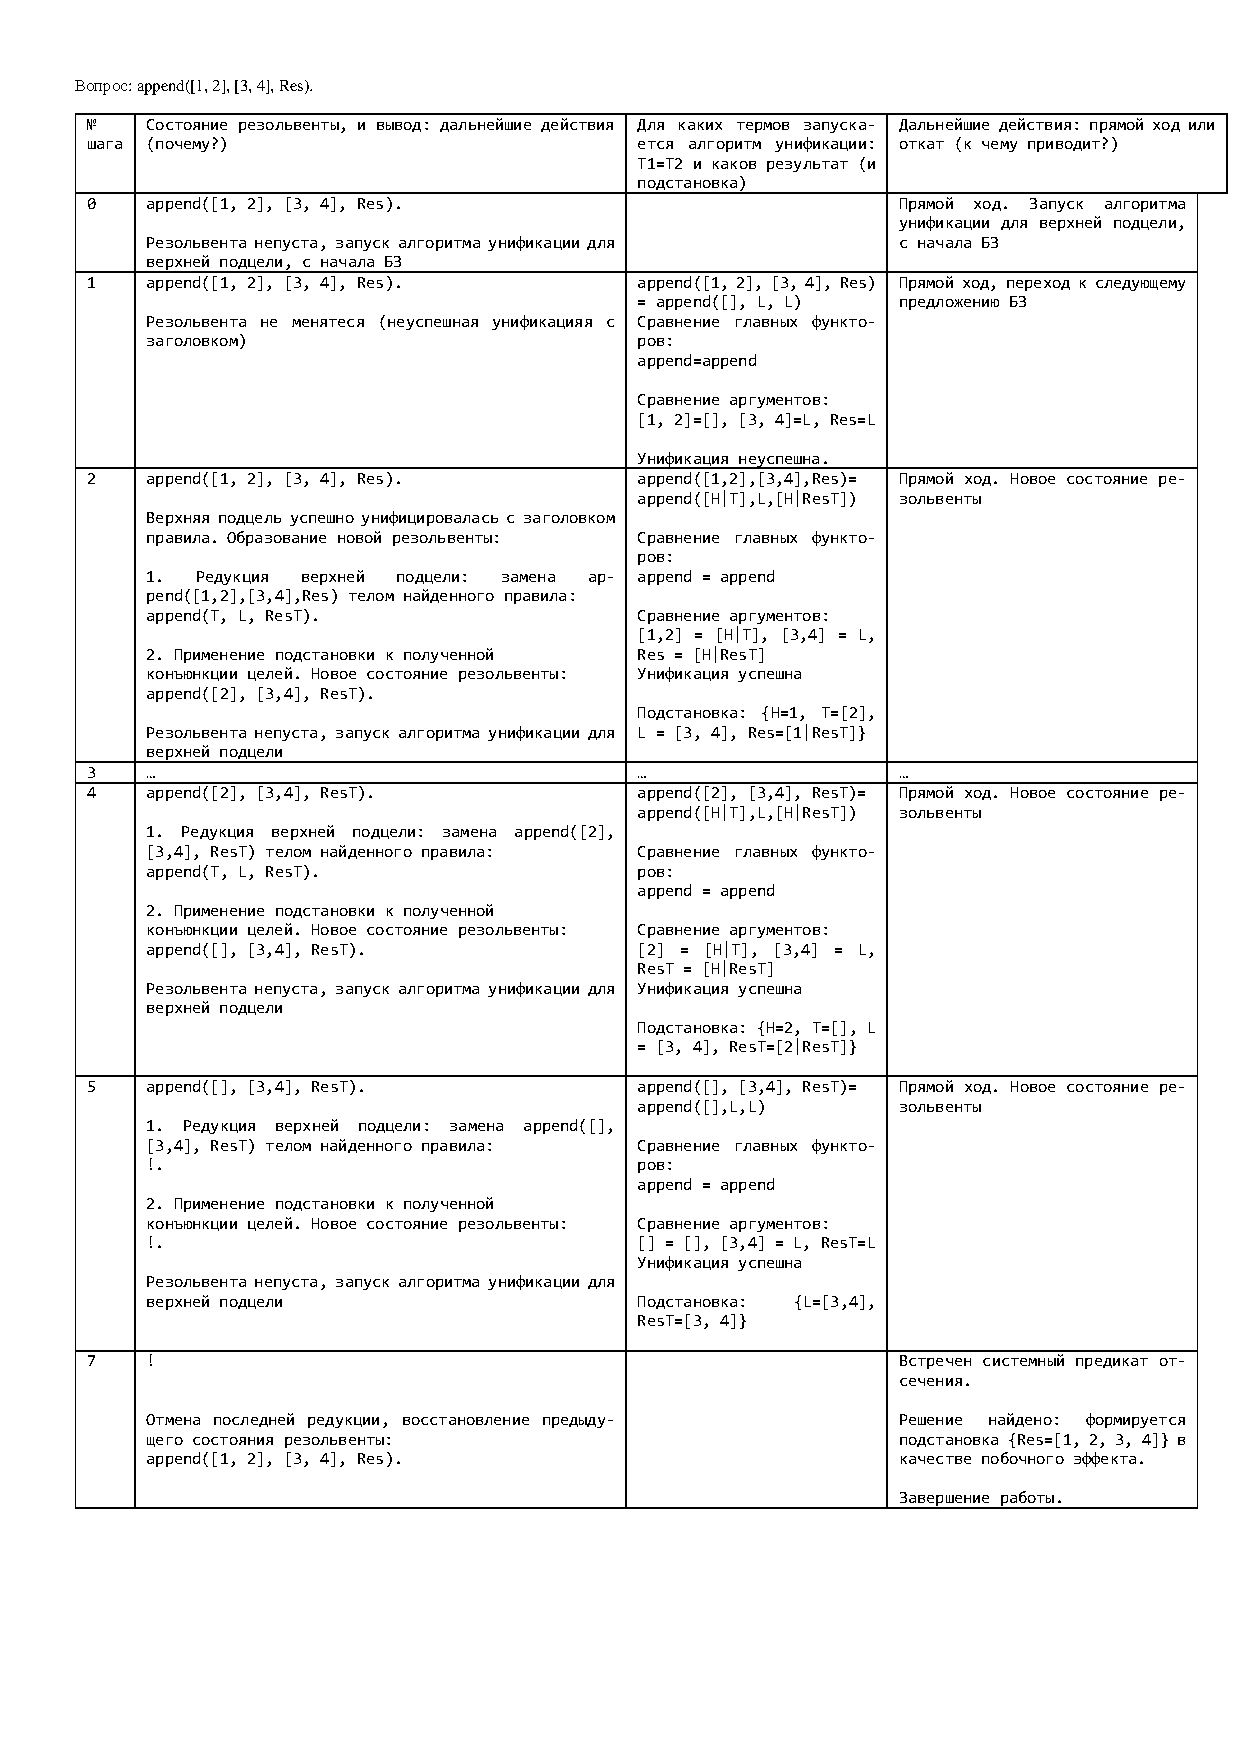
\includepdf{reportT.pdf}
	\bibliographystyle{utf8gost705u}  % стилевой файл для оформления по ГОСТу
	\bibliography{51-biblio}          % имя библиографической базы (bib-файла)
	
\end{document}